\makeatletter \@ifundefined{rootpath}{\input{../../setup/preamble.tex}}\makeatother
\worksheetstart{Roslyn}{0}{Februar 10, 2015}{}{../../}
This chapter presents a conceptual overview of the Roslyn project. In BLA we describe BLA\toby{Ændre dette når vi ved hvad der skal være i kapitlet}

\section{Introduction}
Project Roslyn is Microsoft's initiative of completely rewriting the C\# and \ac{VB} compilers, using their own managed code language. That is, the C\# compiler is written in C\# and the \ac{VB} compiler in \ac{VB}. Roslyn was released as open source at the Microsoft Build Conference 2014\cite{csharpBuild}.

Beyond changing the languages the compilers are written in, Roslyn provides a new approach to compiler interaction and usage. Traditionally a compiler is treated as a black box where it is given source files as input, magic happens in the middle, and out comes objects files or assemblies\cite[p. 3]{ng2012roslyn}. During compilation the compiler builds a deep knowledge about the code, unavailable to the programmer, which is discarded once the compilation is done. This is where Roslyn differs, as it exposes the code analysis of the compiler by providing an \ac{API}, which allows the programmer to obtain information about the different compilation phases\cite[p. 3]{ng2012roslyn}. 

The compiler \acp{API} available are illustrated in \bsref{fig:api_vs_compiler_pipeline} where each \ac{API} corresponds to a phase in the compiler pipeline. In the first phase the source code is turned into tokens and parsed according to the language grammar. This phase is exposed through an \ac{API} as a syntax tree. In the second phase declarations, i.e. namespaces and types from code and imported metadata, are analyzed to form named symbols. This phase is exposed as a hierarchical symbol table. In the third phase identifiers in the code are matched to symbols.\toby{Det inkluderer type check og scope check også?} This phase is exposed as a model which exposes the result of the semantic analysis. In the last phase, information gathered throughout compilation is used to emit an assembly. This phase is exposed as an \ac{API} that produces IL bytecode\cite[p. 3-4]{ng2012roslyn}.
%second phase:  a kind of an index to the sources that tells where namespaces and types are declared

\begin{figure}[htbp]
\centering
 \includegraphics[width=1\textwidth]{\rootpath/worksheets/roslyn/figures/compiler_pipeline_vs_api} 
 \caption{Compiler pipeline in contrast to compiler \acp{API}\cite[p. 4]{ng2012roslyn}.}
\label{fig:api_vs_compiler_pipeline}
\end{figure}

Knowledge obtained through the \acp{API} can be valuable in order to create tools that analyze and transform C\# or \ac{VB} code. Furthermore Roslyn allows interactive use of the languages using a \acs{REPL}\footnote{\url{http://blogs.msdn.com/b/csharpfaq/archive/2012/01/30/roslyn-ctp-introduces-interactive-code-for-c.aspx}}, and embedding of  C\# and \ac{VB} in a \ac{DSL}\cite[p. 3]{ng2012roslyn}.

\section{Inside Roslyn}
In this section we will describe the inner architecture of Roslyn's source code and further elaborate on the compiler phases from \bsref{fig:api_vs_compiler_pipeline}.

\begin{figure}[htbp]
\centering
 \includegraphics[width=0.4\textwidth]{\rootpath/worksheets/roslyn/figures/roslyn_solution_overview} 
 \caption{Overview of projects in Roslyn solution.}
\label{fig:roslyn_solution_overview}
\end{figure}

The Roslyn solution available on github\footnote{\url{https://github.com/dotnet/roslyn}}, forked\footnote{\url{https://github.com/Felorati/roslyn}} on the 9th February 2015, consists of 118 projects which include projects for Visual Studio development, interactive usage of the languages and more as illustrated on \bsref{fig:roslyn_solution_overview}. We will focus on the \bscode{Compilers} folder which contains the source code for the C\# and \ac{VB} compiler, each located in a separate folder. They share common code and functionality within the \bscode{Core} folder which includes code for controlling the overall compilation flow. We describe only the C\# compiler and the core code. However, the code for each compiler is very similar and use the same patterns for compilation\cite[09:36-10:36]{campbellDeeperRos}, so most of the following will apply for the \ac{VB} compiler also.

\begin{figure}[htbp]
\centering
 \includegraphics[width=0.4\textwidth]{\rootpath/worksheets/roslyn/figures/roslyn_csharp_overview} 
 \caption{Overview of CSharp folder.}
\label{fig:roslyn_csharp_overview}
\end{figure}

The projects contained in the \bscode{CSharp} folder are shown on \bsref{fig:roslyn_csharp_overview}. The important projects are \bscode{csc}, \bscode{CSharpCodeAnalysis.Portable} and \bscode{CSharpCodeAnalysis.Desktop}. The \bscode{csc} project is the C\# command line compiler, which is the starting point of a C\# compilation. The two other projects contain the actual code required for compilation. The rest of the projects in the \bscode{CSharp} folder mainly involves tests for the C\# compiler.

In \bsref{fig:roslyn_invoke_overview} an overview of the compilation call chain is shown. Compilation starts with \bscode{csc's} main method being invoked, which calls the static \bscode{Run} method on the \bscode{Csc} class. This method creates a new \bscode{compiler} object of type \bscode{Csc}. \bscode{Csc} is a subtype of \bscode{CSharpCompiler}, located in the \bscode{CSharp.CSharpCodeAnalysis.Desktop} project, which again is a subtype of \bscode{CommonCompiler}, located in \bscode{Core.CodeAnalysis}. This means that the creation of the \bscode{compiler} object, calls the constructors of \bscode{Csc}, \bscode{CSharpCompiler} and \bscode{CommonCompiler}. Afterwards the \bscode{Run} method is invoked on the \bscode{compiler} object, which further invokes its parents \bscode{Run} method, which again invokes its parent \bscode{Run} method. Finally the \bscode{RunCore} method in \bscode{CommonCompiler} is invoked, which contains the general code that controls the overall flow of the compiler pipeline, that was illustrated in \bsref{fig:api_vs_compiler_pipeline}. The \bscode{RunCore} method will for the phases at run time call the actual compiler logic for C\# in \bscode{CSharp.CSharpCodeAnalysis.Portable} or \ac{VB} in \bscode{VisualBasic.BasicCodeAnalysis.Portable} through dynamic dispatch.\toby{Er det helt rigtigt? Muligvis kalder den også i noget generelt, som kun er defineret i core, der ikke kalder videre. Tror måske IL emitting, kun har kode i Core - men er også noget i CSharpCodeAnalysis med kodegenerering. Andet eksempel: SemanticModel ligger i Core.}

\begin{sidewaysfigure}[htbp]
\centering
 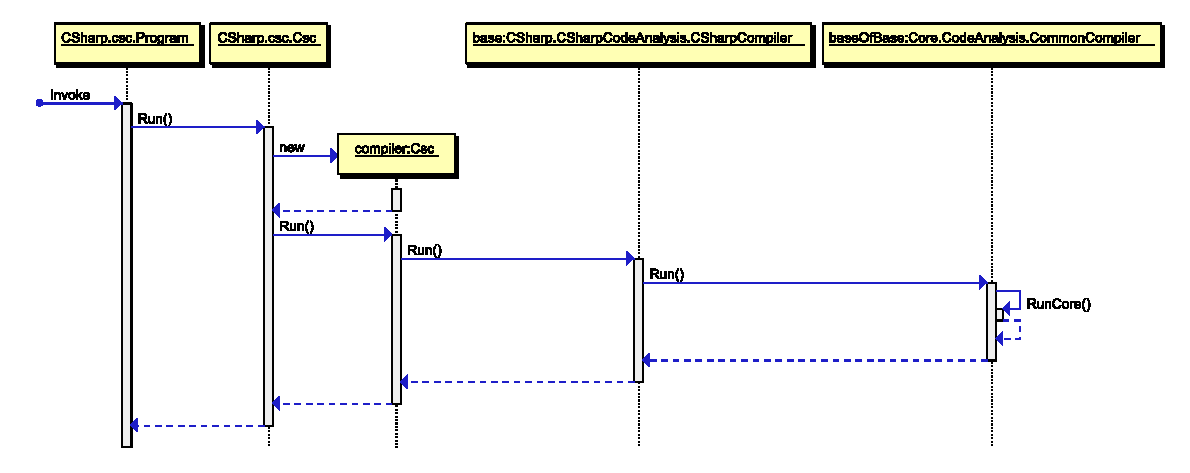
\includegraphics[width=\textwidth]{\rootpath/worksheets/roslyn/figures/seq_diagrams/roslyn_invoke_overview} 
 \caption{Sequence diagram showing an overview of the call chain of a C\# compilation.}
\label{fig:roslyn_invoke_overview}
\end{sidewaysfigure}

\subsection{CSharpCodeAnalysis}
%fortæl om CSharpCodeAnalysis projekterne

\begin{figure}[htbp]
\centering
 \includegraphics[width=0.4\textwidth]{\rootpath/worksheets/roslyn/figures/csharp_codeanalysis_overview} 
 \caption{Overview of the \bscode{CSharp.CSharpCodeAnalysis.Portable} project.}
\label{fig:roslyn_csharpanalysis_overview}
\end{figure}
\toby[i]{Ved ikke om jeg vil have den her figur med}

\section{Key Concepts}
The C\# compiler builds upon concepts from traditional compiler theory, such as lexing, parsing, declaration processing, semantic analysis and code generation\cite{sebestaProLang}\cite{fischer2009crafting}. Throughout the phases of compilation, traditional concepts such as a syntax tree, symbol table and visitor pattern are also used. In this section we describe the core concepts used in the C\# compilation phases.

\subsection{Syntax trees}\label{sec:syntax_trees}
Syntax trees are the primary structure used throughout the phases of compilation. Roslyn's syntax tress have three key attributes\cite[p. 6]{ng2012roslyn}: 
\begin{enumerate}
	\item The first attribute is that a syntax tree is a full fidelity representation of source code, which means that everything in the source code is represented as a node in the syntax tree. If programs are invalid, the syntax tree represent these errors in source code by skipped or missing tokens in the tree. 
	\item The first attribute enables the second attribute, which is that a syntax tree produced from parsing must be round-trippable back to the original source code.
	\item The third attribute is that syntax trees are immutable and thread-safe. This enables multiple users to use the same syntax tree at the same time in different threads without concurrency issues. As syntax trees are immutable, factory methods exists in order to help create and modify trees. This might seem inefficient, as one would expect a copy of the tree is required, however syntax tress are efficient as they reuse underlying nodes. This means that trees can be modified fast and with a low memory overhead. In fact a syntax tree in Roslyn consists of two trees, the red and green tree, which we will now describe.
\end{enumerate}

\subsubsection{Red And Green Trees}\toby{Hvad med boundtree? Eller evt. fortæl om det i et uddybende compiler fase afsnit}
The Roslyn team wanted a primary data structure for compilation with the following characteristics\cite{lippert2012redgreen}:
\begin{itemize}
	\item Immutable.
	\item Form of a tree.
	\item Cheap access to parent nodes from child nodes.
	\item Possible to map from a node in the tree to a character offset in the source code.
	\item Ability to reuse most nodes in the original tree when modifying trees.\toby{måske brug ordet persistent}
\end{itemize}
However fitting all those characteristics into a single data structure is problematic\cite{lippert2012redgreen}. One problem is simply constructing a tree node, as the child and parent must refer to each other, and are immutable, it is not possible to create one before the other. Another problem is reusing nodes for another parent when modifying the tree, as nodes are immutable and it is therefore not allowed to change the parent of a node. A last problem is inserting a new character into the source code, as the position of all nodes after that point changes. This is problematic in relation to adhering to the characteristic of reusing nodes, because a modification to source code can change the character offset of many nodes.
%til den sidste, husk at de selv bruger roslyn til at udvikle interne værktøjer, derfor er det vigtigt at når man skrive et nyt tegn i starten af source koden, at de ikke skal bygge træet helt på nyt.

Instead Roslyn uses two types of trees, green trees and red trees, in order to fulfill all their characteristics.

\paragraph{The green tree} is immutable, has the ability upon modification to reuse most unaffected nodes, has no parent references, is built bottom-up, and knows not the absolute positions of nodes in source code but only their widths\cite{lippert2012redgreen}.

For the expression ``5+5*5+5'', a typical parse tree is shown in \bsref{fig:normal_syntax_tree}, and a potential green tree is shown in \bsref{fig:green_syntax_deduplication}. As the green tree nodes does not have parent references and positions in source code, sub-trees and nodes can be reused, which results in a more compact tree. Factory methods are used to create new nodes in the tree in order to determine if existing nodes can be reused or new ones must be created. If nodes for a given expression already exists they are reused, and otherwise new nodes are created. 

However reuse of existing nodes is not guaranteed, as that requires all nodes to be cached, which makes the reuse caches unnecessarily big. The caches are instead a fixed size, where new nodes will replace older ones when the max size is reached. This does however still work pretty well due to the fact that often recently accessed nodes are likely to be accessed in the near future again\cite{sadovRoslynPerf}. Another trade-off is that they do not reuse non-terminals with more than 3 children, as it gets more expensive and less likely to match, the more children a non-terminal has\cite{sadovRoslynPerf}.\toby{Måske bliver det her for specifikt?}

\begin{figure}[htbp]
\centering
 \includegraphics[width=\textwidth]{\rootpath/worksheets/roslyn/figures/normal_syntax_tree} 
 \caption{Typical parse tree of expression.}
\label{fig:normal_syntax_tree}
\end{figure}

\begin{figure}[htbp]
\centering
 \includegraphics[width=0.6\textwidth]{\rootpath/worksheets/roslyn/figures/green_syntax_deduplication} 
 \caption{Green tree of expression, reusing identical sub-trees. Inspired by \cite{sadovRoslynPerf}.}
\label{fig:green_syntax_deduplication}
\end{figure}

\paragraph{The red tree} is an immutable facade built around the green tree. It has parent references and knows the absolute positions of nodes in source code. However these features prevents nodes from being reused, which means that making modifications to a red tree is expensive. Therefore they take another approach than building a new red tree upon every modification\cite{lippert2012redgreen}. 

The red tree is build lazily using a top-down approach, starting from the root of the tree and descending down into children. To access a given node in the tree, the parent must first be available, otherwise the parents parent must be available, and so on. Once the parent of a node is available, all information required to construct a red node is available. The parent reference is known, as it is the current node. Additionally the internal data for the child can be obtained from the corresponding green node. Furthermore the absolute position of the node in source code can be computed, as the position of the parent is known, and the width of all children that come before the given node\cite{sadovRoslynPerf}.

So when modifications are made to source code, an entire new red tree is not computed. Instead the green tree is modified, which is a relatively cheap operation, as most nodes can be reused. In terms of the red tree, a new root red note is created with 0 as position, null as parent and the root green node as the corresponding green node. The red tree will then only build itself if a user descends into its children, which may not happen and it might only descend into a small fraction of all the nodes in the tree\cite{sadovRoslynPerf}. % i forhold til hvad det er godt til? med ide typing tankegang

\subsection{Contents Of Syntax Trees}
The elements contained within syntax trees are syntax nodes, tokens and trivia. We will in this section describe these and some of their properties.\toby{Evt. nævn spans, kind osv. også}

\subsubsection{Syntax Nodes}
Syntax nodes represent non-terminals of the language grammar, such as declarations, statements and expressions. It is one of the main elements of syntax trees and each syntax node type is represented as a separate class that derives from a base \bscode{SyntaxNode} class.

As syntax nodes are non-terminals, they always have children, either in the form of other syntax nodes or syntax tokens. In relation to navigating the tree all syntax nodes has, a parent property to obtain the parent node, a \bscode{ChildNodes} method to return a list of all child nodes, and descendant methods i.e. \bscode{DescendantNodes}, \bscode{DescendantTokens} and \bscode{DescendantTrivia}, to obtain a list of all descendant nodes, tokens or trivia for a given node. Furthermore, for a given node, each child is also exposed through a separate property\cite[p. 7]{ng2012roslyn}.

Additionally, optional children are allowed, which are represented as \bscode{null} if they are not present. For example an \bscode{IfStatementsyntax} syntax node has an optional \bscode{ElseClauseSyntax} syntax node\cite[p. 7]{ng2012roslyn}.

\subsubsection{Syntax Tokens}
Syntax tokens represent terminals of the language grammar, such as keywords, literals and identifiers. Opposed to syntax nodes, syntax tokes do not have any children. 

Each syntax token does not have a separate class, instead all syntax tokens are represented by a single \bscode{SyntaxToken} type. This means that there is a single structure for all tokens. To get the value of a token, there exists three properties: \bscode{Text}, \bscode{ValueText} and \bscode{Value}. The first returns the raw source text as a \bscode{String}, this includes extra characters such as escape characters. The second returns only the value of the token as a \bscode{String}. The last returns the value as the actual value type e.g. if the token is an integer literal then the property returns the actual integer. To allow different return types, the return type of the last property is \bscode{Object}.

Additionally, for performance reasons the \bscode{SyntaxToken} type is defined as a struct, which is a value type\cite[p. 7]{ng2012roslyn}.

\subsubsection{Syntax Trivia}
Syntax trivia represent extra parts of source code that can appear between any two tokens, such as white space and comments. Syntax trivia is not included as a child node in the tree, but is instead associated with a given token. In general, a token holds all trivia that follows it, on the same line, up to the next token. Syntax tokens hold trivia in two collections: \bscode{LeadingTrivia} and \bscode{TrailingTrivia}. The first token holds all leading initial trivia, and the end-of-file token holds the last trailing trivia in source code\cite[p. 8]{ng2012roslyn}.

As trivia are not nodes in the tree, they do not have a \bscode{Parent} property. Instead the associated token for some trivia, can be accessed with the \bscode{Token} property. Additionally, like syntax tokens, trivia are also value types and have only a single \bscode{SyntaxTrivia} type to describe them all.

\subsubsection{Spans}
Every node, token and trivia knows its position in source code. This is accomplished by the use of a \bscode{TextSpan} struct type. A \bscode{TextSpan} object holds the start position of a node, token or trivia in source code and a count of how long it spans, both as 32-bit integers\cite[p. 8]{ng2012roslyn}.

Every node, token and trivia has two properties to obtain spans: \bscode{Span} and \bscode{FullSpan}. The \bscode{Span} property includes only the span of the node, token or trivia and not any trivia, where the \bscode{FullSpan} property includes the normal span and any leading or trailing trivia.  

\subsubsection{Kinds}
Every node, token and trivia has an integer \bscode{RawKind} property, used to identify the syntax element type. Each language, C\# or \ac{VB}, then contains a \bscode{SyntaxKind} enumeration that contains all the nodes, tokens and trivia in the language, that the integer can be cast to. The \bscode{CSharpSyntaxKind} method does the casting automatically\cite{roslynwikiOverview}\cite[p. 9]{ng2012roslyn}.

Kinds are especially important for tokens and trivia, as they have only a single type,\bscode{SyntaxToken} and \bscode{SyntaxTrivia}, for all tokens and trivia. Thus, the only way to identify the particular token or trivia at hand, is by using kinds.

\subsubsection{Errors}
If programs are invalid as a result of errors in source code, a syntax tree is still produced. These errors are represented as special tokens in the syntax tree, which are added using one of the following techniques\cite[p. 9]{ng2012roslyn}.

One technique is to insert a missing token in the syntax tree when the parser scans for a particular token but does not find it. The missing token represents the expected token, but it has an empty span and has a true \bscode{IsMissing} property.

Another technique is to skip tokens until the parser finds a token where it again can parse. The skipped tokens are added as a trivia node with the \bscode{SkippedTokens} kind.

\subsection{Compilation}
\subsection{Symbols}

%semantic model evt. (tror kun det er i forhold til api)
	%følgende sker direkte i runcore kald
%compilation = source files, assembly references and compiler options. Main: symbol table
	%består af symboler (Symbol klassen)
	
	%måske sker den semantiske analyse i analyzedriver kaldet, eller GetDeclarationDiagnostics()
%semantic model = semantisk analyse, så som type og scope checking, 
	%kan obtains udfra en compilation
	%MERE:
	%The symbols referenced at a specific location in source.
	%The resultant type of any expression.
	%All diagnostics, which are errors and warnings.
	%How variables flow in and out of regions of source.
	%The answers to more speculative questions.
	
%selve emitting sker også i runcore
	%data flow analyse, Control flow analysis også en del af emit (refer til deres paper det ligger på gitten omkring data flow)

\section{Compile Phases}\toby{Måske ryk den op over hvor syntax træer bliver forklaret}\toby{Måske bare være et underpunkt i Inside Roslyn - afhæning af hvor stort afsnittet bliver (evt. kan det komme som det første i inside roslyn)}
%måske noget pre , evt. med at faserne vist i den første figur er simplicifeceret og her vi her er lidt mere uddybende
%refer til VSadov

%evt fortæl ud fra mapperne i projektet?

The first phase of compilation entails initial work, such as parsing the command line with associated parameters and setting up for compilation, as shown in \bsref{fig:roslyn_invoke_overview}.\toby{bedre slutning på sætning}

The second phase involves parsing the source code, which is done in a traditional compiler fashion by lexing source code into tokens and parsing them into a syntax tree, which represents the syntactic structure of the source code. This phase will check for syntax errors in source code, but does not have enough information to check for semantic errors, such as scope or type errors.
%special type syntax tree, refer til det blvier beskrevet senere hvis det rykkes op
%ligger i parse mappen: Lexer.cs + SyntaxParser (der er også LanguageParser.cs og DirectiveParser.cs) 
%recursive descent parser
%first phase on fig. 1.1

%Syntax trees represent the lexical and syntactic structure of source code. Although this information alone is enough to describe all the declarations and logic in the source, it is not enough information to identify what is being referenced.

%a semantic model encapsulates the language rules, giving you an easy way to make these distinctions.

In order to obtain more information, IN BLA creates a declaration table, which takes the form of a tree, that holds where namespaces and types are declared in source code.
	%åbenbart en del af en compilation
	
%Compilation object, which is 

%types and namespaces
%namespaces, classes, interfaces, structs, and delegate declarations

%second phase on fig 1.1 (tror jeg) - skal være sikker på hvad symbols er
%forklaret mere om den i CSharp > CSharpCodeAnalysis (Portable) > Declarations > Declaration.cs og DeclarationTable.cs (Table indeholder forskellige typer af Declaration, såsom SingleTypeDeclaration)

%second, declration phase: declarations from source and imported metadata are analyzed to form named symbols.
	%the declaration phase as a hierarchical symbol table
	%åbenbart både declaraiton og symbol table?

%***Mangler hvad fase 2 er i fig.1.1, eller hvor det sker præcist.

The fourth phase declaration diagnostics (fase 3 i fig 1.1)
%third phase of fig 1.1 (fully bind)
%resultatet er et bound træ, hvilket er en internal repræsentation for Roslyn (som ikke er tilgængelig igennemt API'et)
%symbol visitor sker heri (men den tager et symbol, så det må ske før)

The fifth IL emitting
%the fourth

The sixth serialization of portable executable file and pdb file (used for debugging).

%pdb info:
	%http://www.wintellect.com/devcenter/jrobbins/pdb-files-what-every-developer-must-know

%et sted skal scope og type tjek checkes

%secon phase on fig 1.1


%evt. lav en figur over disse faser

%sequential



%\toby[i]{Skal have det et sted, hvor jeg fortæller mere præcist en compiler line billedet om faserne der sker, ligesom beskrevet i blogpostet. Evt. også i forhold til om de køres med en eller flere tråde}
%Earlier in intro we looked at the phases of the compiler in contrast to the compiler API, howerver This does not include all phases. In this section we will explain in more detail what phases the compiler consits of and how it is build on in the code
	%Omformuler så det lyder bedere (men noget i den stil)

%Forklar de forskellige kompilerigns faser

%overordnet beskrivelse af faserne og evt. hvis api i forhold til også
	%ved ikke om jeg skal bruges deres tegning eller lave en ny selv (eller begge dele)

%snak ikke om det under white paper underskriften: API Layers

%MORE:

%Known Limitations and Unimplemented Language Features
	%https://social.msdn.microsoft.com/Forums/vstudio/en-US/f5adeaf0-49d0-42dc-861b-0f6ffd731825/known-limitations-and-unimplemented-language-features?forum=roslyn

%Liste over mulige emner:
	% Beskrivelse af kompileren, og hvad de muliggøre med deres API.
	% De enkelte faser i kompileren og generelt om dens opbygning
	% Hvilke ting de har gjort i forhold til at forbedre performance
	% Fortælle om deres røde og grønne syntaks træ
	% De anvender traditionel compiler teori, med lexer og parser + syntaxtræ og visitor til at traverserer træet. og emit fase.
	%Evt. fortæl om faserne i forhold til mapperne i projektet. Med Core, VB og C# projekternere og til sidst fortæl udfra C#'s mapper (og de forskellige faser).
	%Evt. også nævn syntax visualizer (nok ikke så vigtig, men er et værdifuldt værktøj)
	%Immutable data struktuerer!
	%Hvilke muligheder man har for at implementere STM direkte i Roslyn
		%Ved hjælp af API, hvor vi gør det først og derefter fodrer output til csc.exe
		%Direkte i compileren.


%Den primære brug der er tiltænkt at programmøren skal få adgang er gennem API laget, hvor en del kompleksitet stadig er gemt væk.
	%Vi vil gå direkte ind og ændre i selve compileren, hvilket ikke er tiltænk som hovedtanken fra Microsoft's side.
	
%Evt. skriv at vi vil have fokus på syntax træet og går mest i detalje med det, fordi vores implementering har valgt at ændre i syntax træet.
	%men alligevel kort om de andre faser.
\worksheetend